\section{Gestion de version}

\begin{frame}{Gestion de version : concepts}
Lorsqu'on travaille sur une projet (seul ou à plusieurs) il est souhaitable de pouvoir :
\begin{itemize}
\item avoir des copies de son travail
\item revenir à des version précédentes
\item faciliter la parallélisation du travail
\end{itemize}

Un gestionnaire de version permet cela.
\end{frame}

\begin{frame}{Gestionnaire de version  en client-serveur}{CVS, Subversion}
\begin{center}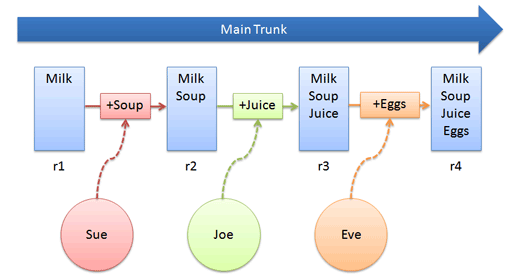
\includegraphics[scale=0.6]{centralized_example.png}\end{center}
\end{frame}

\begin{frame}{Gestionnaire de version distribué}{Bazaar, git, Mercurial}
\begin{center}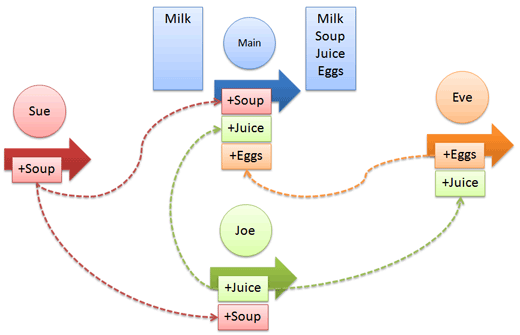
\includegraphics[scale=0.6]{distributed_example.png}\end{center}
\end{frame}

\begin{frame}{Comparaison}
\includemedia{La vidéo ne marche pas}{centralized-vs-distributed.mp4}
\end{frame}

%http://betterexplained.com/articles/intro-to-distributed-version-control-illustrated/

